\label{sec:introduction}
\textit{Author: Marina Mursa}

In this introductory Chapter the rationale for this study is explained and an overview of the project is provided.  It states the motivation behind the research, follows through with the goals that were set to be accomplished by the framework as well as the faced challenges. It finishes by giving an overview of the structure of this report.

\section{Motivation}
In a world hooked on technologies, a connection to the outside world is crucial, even during driving. This is the reason why the majority of car manufacturers try to come up with some technological ecosystem/framework that would connect the car and the user to the world around him.\\
BMW technology package called \emph{ConnectedDrive} has currently over 8 million cars that connect daily to almost 300 micro services that guarantee not only entertainment but most importantly the security of the users. This services range from Map Updates and Real Time Traffic Information to Concierge Services. Due to such a diversity of services as well as the constantly growing number of worldwide users, the cars become moving data centers.\footnote{For more information about ConnectedDrive  see \url{https://www.bmwoffreeport.com/blogs/827/what-is-bmw-connecteddrive/}}\\
For a car to have access to the above mentioned services it requires to make a connection to the BMW servers. Aggregating these connections by time, one type of data that results is represented in the form of requests to connect to BMW servers per second \textbf{(requests/sec)}. Each time a service is interacted with, a request is registered, this way, the data is generated continuously. It's worth noting that there exist only a few BMW data centers worldwide that handle this type of information. They are divided in geographical regions like Australia, USA and Europe. The last one includes not just the Continental Europe, but basically the rest of the globe, excluding the first two regions. This indicates how big the amount of handled data is.\\
The visualisation of such data can be seen in Fig. \ref{fig:data_graph}.
\begin{figure}[h]
    \centering
    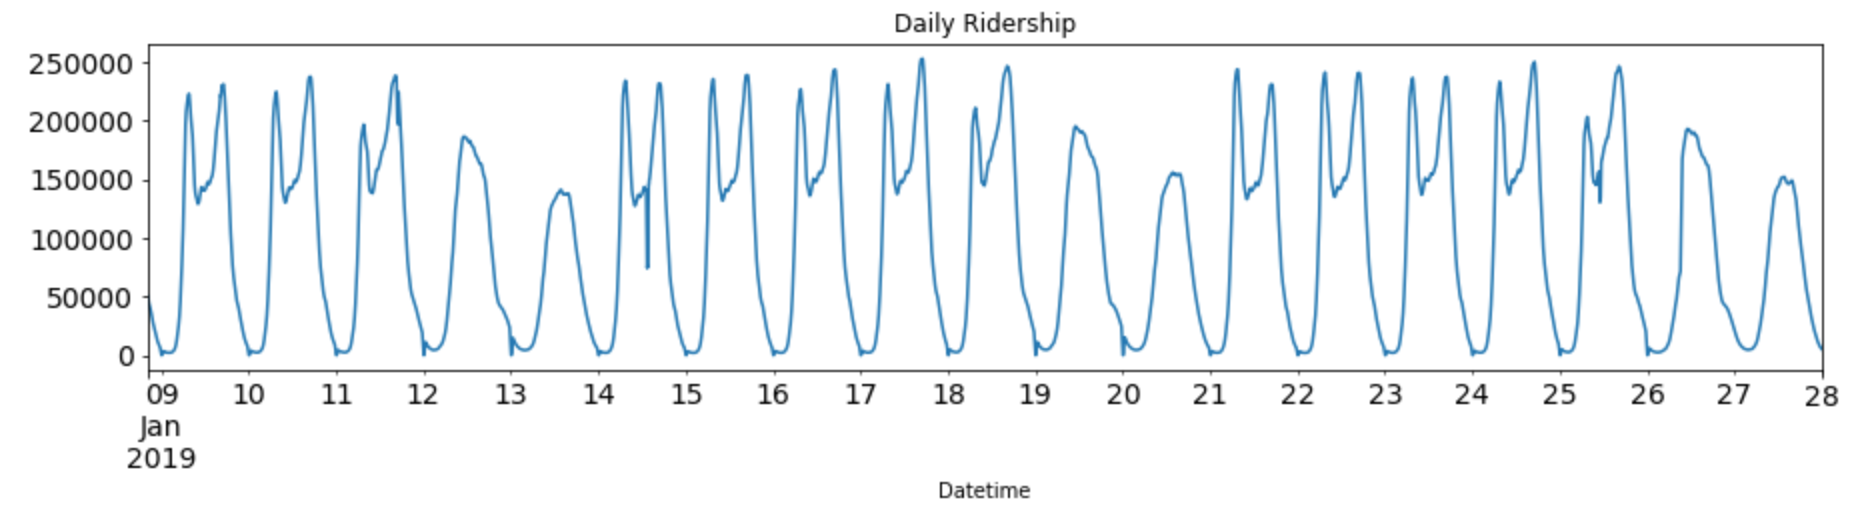
\includegraphics[width=1\textwidth]{images/data_graph.png}
    \caption{Visualisation of BMW data in form of requests per second }
    \label{fig:data_graph}
\end{figure}
\\
A closer inspection of the graph can reveal the following insights:
\begin{enumerate}
    \item A daily pattern can be observed that corresponds to the intuitive rush-hour peaks. One can notice those elevations around the expected 7:30 and 18:00 (+/- 30 min).
    \item A week pattern emerges, where the week days (Monday through Friday) have a strong resemblance, and the weekend days (Saturday and Sunday) have a a slightly changed, more Gaussian pattern.
\end{enumerate}

Having such huge amounts of data generated every second, one wonders how can it bring more value to the framework. This way, the challenge of this project was to identify ways to extract that hidden existing knowledge. 

\section{Use Cases}
The following section will introduce the two identified use cases for handling the data, the goals that were set for each of them, as well as the challenges each of them pose.
    \subsection{Use Case 1 - Anomaly Detection}
     \label{sec:use_case1}
      Looking back at Fig. \ref{fig:data_graph}, one can observe a drop in the graph on the 14th of January, that deviates from our expectations. Because the data is a representation of the number of requests to connect to the BMW servers, this drop can indicate either a problem that occurred in processing the received requests or an issue in receiving them, like a power breach.  \\
      Being able to identify these deviations that do not correspond to the “normal” distribution of data, would allow The BMW team to react faster in solving the issues behind them. Of course, the faster the anomalies are detected, the quicker the team can intervene, thus assuring that no data is lost due to technical problems, and that the user gets the full ConnectedDrive experience. \\
      
\textbf{Goal}\\
    This way, the goal for this use case is to develop a framework, based on AWS service, that would be able to detect in a real-time environment a deviation from the patterns mentioned above, label it as an \emph{anomaly}, and escalate a notification to a tool, e.g. a Slack channel, in the form of an alert accompanied by a small visual representation of the problem.\\
    To achieve this goal the team challenged itself to explore a couple of machine intelligence solutions that deal with anomaly detection on time series data. After successful implementation, these models should be compared, and based on their advantages and disadvantages one solution should be chosen for the final product.\\
    
\textbf{Challenges}\\
    Analyzing the goal and trying to break it down into smaller tasks revealed a couple of challenges that the project would have to deal with prior to starting the actual developing process. These questions are:
\begin{enumerate}
 	\item\emph{How do we define normal?} As it was mentioned above, an anomaly is described as a deviation from the normal expectation. Taking in consideration the fact that the data is not a linear distribution, but has a specific pattern that changes depending on the hour of the day, stating what normal is becomes difficult.
	\item\emph{How big of a deviation is an anomaly?} As all distributions, this data has a degree of noisiness to it. Making the framework too sensible will result in a high number of notification, while defining the anomalies too broad will only detect major issues.
\end{enumerate}
    The following chapters will offer more details on the issues and the way the project dealt with them both short  and long term.\\
    
\subsection{Use Case 2 - Time series Forecasting}
    \label{sec:use_case2}
    Going back to the the Fig. \ref{fig:data_graph}, one can observe that the number of requests varies highly during the period of a day. This means that the required computational power to process them should follow the same trend. But because the pipeline that processes all the requests is based on AWS services, the scaling of the infrastructure can be done only post-event. This means that for a short period of time the system still uses higher computational power then required, which translates in higher maintenance costs.\\
    A prognosis of the data distribution would allow the BMW team to adapt the infrastructure based on the predicted needs, thus reducing the expenses with the AWS services in a predictive manner.\\
    
    \textbf{Goal}\\
    Thus, the project attempts to incorporate a prediction feature, that would deliver short-term prognosis which would allow for predictive scaling of the infrastructure.\\
    As in the previous use case, the team challenges itself with implementing and comparing a series of solutions. Such an approach offers a better perspective of the issues. Comparing the pluses and minuses of a series of machine intelligence models, gives more confidence in recommending a final solution.\\ 
    
\textbf{Challenges}\\
    As one might intuit, this use case comes with a series of challenges that need to be addressed during the implementation. Such challenges include the following questions: 
    \begin{enumerate}
        \item\emph{How to handle holidays?} As one can see in the following chapters, holidays are an exception in terms of their pattern, so they do not obey the trends that we discussed above.
 	    \item\emph{How far ahead can we predict?} Although for predictive scaling the system would need just the prognosis for a couple of hours, finding out the maximum prediction period  would help determining the limitations of a model.
 	\end{enumerate}
 	The way our goals were achieved, as well as the manner in which these issues were handled and their detailed solutions will be presented in the following chapters.
 	
 	
\section{Outline}
    This report paper is structured in the following way: \\
    Next chapter is a complex one that starts by explaining the \textbf{structure of the system architecture} of the final product of the project. It continues by giving insights into the way the \textbf{data is handled}, detailing also on a temporary solution that was explored in the early stages of the project.\\
    As the project has two main story lines that correspond to each use case, the report continues with \textbf{detailed explanations of the trial models} for each of them, providing a theoretical explanation, implementation example and results of validating the models against the BMW dataset.\\
    The paper continues with explanations about the means the results of the above mentioned machine intelligence model are reported to a responsible party.\\
    And finally, the chapter finished with details on the \textbf{delivery solution}.\\
    The paper continues by describing the way the project was handled from a managerial point of view. And finishes with a list of recommendations.